\documentclass{scrreprt}

\usepackage{aligned-overset}
\usepackage{amsmath}
\usepackage{amssymb}
\usepackage{bm}
\usepackage[shortlabels]{enumitem}
\usepackage{hyperref}
\usepackage[utf8]{inputenc}
\usepackage{multicol}
\usepackage{mathtools}
\usepackage{physics}
\usepackage{tabularx}
\usepackage{titling}
\usepackage{fancyhdr}
\usepackage{xfrac}
\usepackage{pgfplots}

\pgfplotsset{compat = newest}
\usetikzlibrary{intersections}
\usetikzlibrary{patterns}
\usepgfplotslibrary{fillbetween}

\author{Karsten Lehmann}
\date{WiSe 2021/2022}
\title{Übungsblatt 02\\Analysis - Grundlegende Konzepte}

\setlength{\headheight}{26pt}
\pagestyle{fancy}
\fancyhf{}
\lhead{\thetitle}
\rhead{\theauthor}
\lfoot{\thedate}
\rfoot{Seite \thepage}

\begin{document}
\paragraph{6. Es werden die folgenden Aussagen betrachtet:}
\begin{enumerate}[label={(A\arabic*)}]
\item ``Jede:r Studierende kann beim Hören jedes Musikstücks mindestens
  eine Hausaufgabe lösen.''
\item ``Es gibt (mindestens) eine:n Studierende:n und (mindestens) ein
  Musikstück, sodass diese:r Studierende beim Hören dieses Stückes alle
  Aufgaben lösen kann.''
\end{enumerate}

Drücken Sie die beiden Aussagen mit den Quantoren $\forall$ und $\exists$ aus.
Beschreiben Sie dazu die Studierenden, Musikstücke und Hausaufgaben durch Mengen.
Negieren Sie anschließend die beiden Aussagen.
Dabei soll die Negation von (A1) nicht mit ``Nicht zu jedem'' beginnen,
und die Negation von (A2) nicht mit ``Es gibt keine''.
Formulieren Sie im Anschluss die negierten Aussagen wieder in natürlicher
Sprache.

\subparagraph{Lsg.} Sei $S$ die Menge der Schüler, $M$ die Menge der Musikstücke
und $H$ die Menge der Hausaufgaben.
Weiterhin beschreibt die Aussage $P(s, m, h)$, dass der Schüler $s$
beim Hören des Musikstückes $m$ die Hausaufgabe $h$ lösen kann.

\begin{enumerate}[label={(A\arabic*})]
\item $\forall \, s \in S \colon \forall \, m \in M \colon \exists \, h \in H \colon P(s, m, h)$

  \textbf{Negation}: $\exists \, s \in S \colon \exists \, m \in M \colon \forall h \in H \colon \neg P(s, m, h)$

  ``Es gibt mindestens einen Schüler, für den mindestens ein Musikstück
  existiert, bei dem der Schüler nicht in der Lage ist, irgendeine Hausaufgabe
  aus dem Kurs zu lösen.''

\item $\exists \, s \in S \colon \exists \, m \in M \colon \forall \, h \in H \colon P(s, m, h)$

  \textbf{Negation}: $\forall \, s \in S \exists \, h \in H \colon \colon \forall \, m \in M \colon \neg P(s, m, h)$

  ``Für alle Schüler existiert (mindestens) eine Hausaufgabe, die der Schüler
  beim Hören von Musik (egal welches Stück) nicht lösen kann.''
\end{enumerate}

\paragraph{7. Sei $A$ eine Menge von Parteien, $B$ eine Menge von Wahlversprechen
  und $C$ die Menge der Wahlen.}
Weiterhin ist $P(a, b, c)$ die Aussage
\begin{center}
  ``Partei $a$ löst das Wahlversprechen $b$ zur Wahl $c$ nicht ein.'' 
\end{center}

Diskutieren Sie den Unterschied der folgenden Aussagen:
\renewcommand{\theequation}{\arabic{equation}}
\begin{align}
  \forall \, a \in A \colon \exists \, b \in B \colon \forall \, c \in C &\colon P(a, b, c) \\
  \forall \, a \in A \colon \forall \, c \in C \colon \exists \, b \in B &\colon P(a, b, c)
\end{align}

\subparagraph{Lsg.}
Die erste Aussage besagt, dass jede Partei mindestens ein Wahlversprechen hat,
welches noch bei keiner Wahl eingehalten wurde.
Die zweite Aussage hingegen besagt, dass jede Partei bei jeder Wahl mindestens
ein Wahlversprechen bricht.

\newpage
\paragraph{8. Seien $A$, $B$ und $C$ Aussagen. Sind die folgenden Aussagen Tautologien?}

\begin{enumerate}[a)]
\item $\qty\big(A \Rightarrow B) \iff \neg \qty\big(A \land \neg B)$

  \subparagraph{Lsg.} durch Wahrheitstabelle
  \begin{center}
    \begin{tabular}{c | c | c | c | c}
      $A$ & $B$ & $A \Rightarrow B$ & $\neg(A \land \neg B)$ & a) \\
      \hline
      W & W & W & W & W \\
      W & F & F & F & W \\
      F & W & W & W & W \\
      F & F & W & W & W
    \end{tabular}
  \end{center}
  $\Rightarrow$ ist eine Tautologie.

\item $\qty\Big(\qty\big(A \land B) \Rightarrow C) \iff \qty\big(C \lor \neg B \lor \neg A)$

  \subparagraph{Lsg.} Der Ausdruck $C \lor \neg B \lor \neg A$ ist genau dann
  falsch, wenn $C = $ F und $A = B = $ W.
  In diesem Fall ist auch $\qty\big(A \land B) \Rightarrow C$ falsch.

  Angenommen $A$ und/oder $B$ wären falsch, dann sind $(A \land B) \Rightarrow C$
  und $C \lor \neg B \lor \neg A$ unabhängig vom Wert von $C$ immer wahr.

  Sei nun $A$, $B$, $C$ wahr, dann ist auch die Aussage wahr.

  \begin{center}
    \begin{tabular}{c | c | c | c | c | c}
      $A$ & $B$ & $C$ & $(A \land B) \Rightarrow C$ & $C \lor \neg B \lor \neg A$ & b) \\
      \hline
      W & W & F & F & F & W \\
      W & F &   & W & W & W \\
      F & W &   & W & W & W \\
      W & W & W & W & W & W
    \end{tabular}
  \end{center}
  $\Rightarrow$ ist eine Tautologie.

\item $\qty\big(A \iff B) \iff \neg \qty\Big(\qty\big(A \land B) \lor \neg A \lor \neg B)$
  \subparagraph{Lsg.} Seien $A$ und $B$ wahr.
  Dann ist die Aussage $A \iff B$ wahr.
  Auch $(A \land B) \lor \neg A \lor \neg B$ ist dann wahr.
  Somit ergibt sich $W \iff F$ und damit ist die Aussage keine Tautologie.
\end{enumerate}

\newpage
\paragraph{9. Seien $M$ eine Menge und $P$, $Q$, $R$ Teilmengen von $M$.}

\begin{enumerate}[a)]
\item Beweisen Sie das Distributivgesetz
  \[
    \qty\big(P \cup Q) \cap R = \qty\big(P \cap R) \cup \qty\big(Q \cap R)
  \]

  \subparagraph{Lsg.} Zwei Mengen $A$ und $B$ sind gleich, genau dann wenn
  $A \subset B \land B \subset A$.

  $x \in A \cup B \iff x \in A \lor x \in B$

  $x \in A \cap B \iff x \in A \land x \in B$
  \begin{itemize}
  \item[``$\Rightarrow$''] Sei nun $x \in \qty\big(P \cup Q) \cap R$.
    Das heißt $x$ ist in $R$ enthalten \textbf{und} $x$ ist in $P$ und/oder
    $Q$ enthalten.
    \[
      x \in R \land \qty\big(x \in P \lor x \in Q)
    \]
    Anders geschrieben: $x$ ist in $R$ und $P$ enthalten \textbf{und/oder}
    $x$ ist in $R$ und $Q$ enthalten.
    \[
      \qty\big(x \in R \land x \in P) \lor \qty\big(x \in R \land x \in Q)
    \]
    $\Rightarrow x \in \qty\big(P \cap R) \cup \qty\big(Q \cap R)$

    $\Rightarrow \qty\big(P \cup Q) \cap R \subset \qty\big(P \cap R) \cup \qty\big(Q \cap R)$

  \item[``$\Leftarrow$''] Sei nun $x \in \qty\big(P \cap R) \cup \qty\big(Q \cap R)$.
    Das heißt $x$ ist in $R$ und $P$ enthalten \textbf{und/oder} $x$ ist in $R$ und
    $Q$ enthalten.
    \begin{align*}
      x \in \qty\big(P \cap R) &\lor x \in \qty\big(Q \cap R) \\
      \qty\big(x \in P \land x \in R) &\lor \qty\big(x \in Q \land x \in R)
    \end{align*}
    Anders geschrieben: $x$ ist in $R$ enthalten \textbf{und} $x$ ist in $P$ und/oder
    $Q$ enthalten.
    \[
       x \in R \land \qty\big(x \in P \lor x \in Q)
    \]
    $\Rightarrow \qty\big(P \cap R) \cup \qty\big(Q \cap R) \subset \qty\big(P \cup Q) \cap R$
  \end{itemize}

\item Beweisen Sie
  \[
    \qty\big(P \setminus Q) \setminus R \subset P \setminus \qty\big(Q \setminus R)
  \]
  \subparagraph{Lsg.} Grafische Lösung

  \begin{minipage}[t]{.4\textwidth}
    \begin{tikzpicture}[remember picture]
      \begin{scope}
        \clip (1, 0) circle (1cm);
        \fill[even odd rule, color=green!30]
            (2.5, 0) circle (1cm)
            (1, 0) circle (1cm);
      \end{scope}
      \begin{scope}
        \path[clip] (2.5, 0) circle (1cm) [insert path={(2, -2) -- (0, -2) -- (0, 2) -- (2, 2)}];
        \path[clip] (1.75, -1) circle (1cm) [insert path={(2, -2) -- (0, -2) -- (0, 2) -- (2, 2)}];
        \fill[pattern color=blue, pattern=north west lines]
            (1, 0) circle (1cm);
      \end{scope}
      \node at (0, 1.3) (label_p) {$P$};
      \node at (3.3, 1.3) (label_q) {$Q$};
      \node at (3.3, -1.5) (label_r) {$R$};
      \node[black!30!green] at (0, -2) (label_pq) {$P \setminus Q$};
      \node[blue] at (-1, -1) (label_pqr) {$\qty(P \setminus Q) \setminus R$};
      \node[circle, draw, minimum size=2cm] at (1, 0) (set_p) {};
      \node[circle, draw, minimum size=2cm] at (2.5, 0) (set_q) {};
      \node[circle, draw, minimum size=2cm] at (1.75, -1) (set_r) {};
      \draw[->] (label_p) -- (set_p.center);
      \draw[->] (label_q) -- (set_q.center);
      \draw[->] (label_r) -- (set_r.center);
      \draw[->,black!40!green] (label_pq) -- (1, -0.6);
      \draw[->,blue] (label_pqr) -- (0.3, -0.2);
    \end{tikzpicture}
  \end{minipage}
  \hfill
  \begin{minipage}[t]{.4\textwidth}
    \begin{tikzpicture}
      \fill[pattern color=blue, pattern=north west lines]
          (1, 0) circle (1cm);
      \begin{scope}
        \clip (2.5, 0) circle (1cm);
        \fill[even odd rule, color=green!30]
            (1.75, -1) circle (1cm)
            (2.5, 0) circle (1cm);
      \end{scope}
      \node at (0, 1.3) (label_p) {$P$};
      \node at (3.3, 1.3) (label_q) {$Q$};
      \node at (3.3, -1.5) (label_r) {$R$};
      \node[black!30!green] at (4, -1.2) (label_qr) {$Q \setminus R$};
      \node[blue] at (0, -2) (label_pqr) {$P \setminus \qty\big(Q \setminus R)$};
      \node[circle, draw, minimum size=2cm] at (1, 0) (set_p) {};
      \node[circle, draw, minimum size=2cm] at (2.5, 0) (set_q) {};
      \node[circle, draw, minimum size=2cm] at (1.75, -1) (set_r) {};
      \draw[->,green] (label_qr) -- (2.7, -0.2);
      \draw[->,blue] (label_pqr) -- (0.7, -0.3);
      \draw[->] (label_p) -- (set_p.center);
      \draw[->] (label_q) -- (set_q.center);
      \draw[->] (label_r) -- (set_r.center);
    \end{tikzpicture}
  \end{minipage}

  \newpage
  $x \in \qty(A \setminus B) \iff x \in A \land \neg(x \in B)$

  Sei $x$ ein Element aus $\qty\big(P \setminus Q) \setminus R$.
  \setcounter{equation}{0}
  \begin{flalign}
    x \in \qty\big(P \setminus Q) &\land \neg \qty\big(x \in R) & \\
    \qty\big(x \in P \land \neg \qty(x \in Q)) &\land \neg \qty\big(x \in R) \\
    x \in P &\land \qty\big(\neg \qty(x \in Q) \land \neg \qty(x \in R)) \\
    x \in P &\land \qty\big(\neg \qty(x \in Q) \lor x \in R)) \\
    x \in P &\land \neg \qty\big(x \in Q \land \neg \qty(x \in R)) \\
    x \in P \setminus \qty\big(Q \setminus R)
  \end{flalign}
  \textbf{Anmerkung:} Es gilt $(3) \Rightarrow (4)$.
  Damit $(3)$ wahr ist, darf $x$ kein Element in $Q$ sein.
  Somit ist auch $(4)$ wahr.

\item Zeigen Sie an einem Beispiel, dass die Inklusion echt sein kann.
  Folgt daraus schon, dass die umgekehrte Inklusion im Allgemeinen nicht gilt?

  \subparagraph{Lsg.} Ein Beispiel ist die grafische Lösung aus der Aufgabe b).

  Sei $P = \qty{1, 2, 3, 4}$, $Q = \qty{3, 4, 5}$ und $R = \qty{2, 4, 6}$.
  Dann ist $(P \setminus Q) \setminus R = \qty{1, 2} \setminus R = \qty{1}$ und
  $P \setminus \qty\big(Q \setminus R) = P \setminus \qty{3, 5} = \qty{1, 2, 4}$.

  Daraus folgt jedoch \emph{nicht}, dass die umgekehrte Inklusion nicht gilt.
  So gilt $P \setminus \qty\big(Q \setminus R) \subset
  \qty\big(P \setminus Q) \setminus R$ zum Beispiel für alle $P$ und $Q$
  solange $R = \emptyset$.
\end{enumerate}

\end{document}